\begin{multicols}{3}[\section{Bluetooth 4.0}]

\rhead{Thomas Schaffroth, Mirko Grothe}
\lfoot{17.05.2016}

\newrefsegment

\begin{tabular}{p{2,1 cm}p{2.7 cm}}
\textbf{Steckbrief}& \\
\end{tabular}
\rowcolors{1}{\topicolor!20}{}
\begin{tabular}{p{2,1 cm}p{2.7 cm}}
      Einsatz seit & Juni 2010\\
      Frequenz"-bereich  & \SI{2400}{\giga\hertz}\\
      Datenrate & \SI{1}{MBit/s}\\
      Verbreitung & Weltweit\\
      Reichweite & \SI{10}{\metre}\\
\end{tabular}
\par

\subsection*{Überblick}
\begin{wrapfigure}{r}{0.4\linewidth}
  \vspace{-20pt}
  \begin{center}
  	\hspace{-20pt}
    
\includegraphics[width=0.7\linewidth]{Kapitel/Bluetooth_4/Grafiken/logo.jpg}
  \end{center}
  \vspace{-15pt}
\end{wrapfigure}
Die Bluetooth Technologie wurde im Jahr 1994 als drahtlose Alternative zu Datenkabeln entwickelt. Bluetooth wurde als offener Standard entworfen, um Verbindungen zwischen verschiedenen Produkten möglich zu machen.~\cite{Bluetooth_4.1} Beispiele für die Nutzung von Bluetooth im Alltag sind Freisprechanlagen für Smartphones im Auto, das Telefonieren über Bluetooth-Headsets, das Hören von Musik über einen drahtlosen Lautsprecher oder die Übertragung von Daten zwischen zwei mobilen Geräten. In diesem Artikel werden zu Beginn die Architektur, das Übertragungsverfahren und die Rahmenstruktur von Bluetooth allgemein erläutert, da sich daran in der Spezifikation 4.0 nichts geändert hat. Anschließend wird auf die Neuerungen von Bluetooth 4.0 gegenüber den vorherigen Versionen eingegangen.

\subsection*{Technische Erläuterungen}
\subsubsection*{Architektur der Bluetooth Technologie}
Die Verbindung zwischen Bluetooth Geräten erfolgt über ein Piconetz. Ein Piconetz ist ein \textbf{PAN} (\textbf{P}ersonal \textbf{A}rea \textbf{N}etwork) von Endgeräten, die über Bluetooth miteinander verbunden sind. Unter einem Personal Area Network versteht man ein Netz, das von Kleingeräten wie PDAs oder Mobiltelefonen ad-hoc auf- und abgebaut werden kann. 
Ein Piconetz besteht aus einem Master-Knoten, bis zu sieben aktiven Slave-Knoten, die sich in einem maximalen Umkreis von 10m zum Master befinden, und bis zu 255 geparkten Knoten. Dabei entspricht jeder Knoten einem mobilen Gerät bzw. Teilnehmer. Geparkte Knoten sind Geräte, die der Master in einen Ruhezustand versetzt hat, um den Batterieverbrauch zu senken. In diesem Zustand wird ein Gerät nur durch den Masters wieder aktiviert. Darüber hinaus ist es möglich, mehrere Piconetze über einen Bridge-Knoten zu verbinden. Es entsteht ein sogenanntes Scatternetz (Abb.~\ref{fig:bt4.scatternetz}). In einem Piconetz sind Slaves nicht eigenständig, sondern warten auf Anweisungen durch den Master. Dieser steuert den Takt und entscheidet, wer in welcher Zeitscheibe (Zeitintervall) Daten übertragen darf. Die Kommunikation erfolgt dabei nie von Slave zu Slave, sondern  immer über den Master-Knoten.~\cite{Bluetooth_4.2}

\begin{Figure}
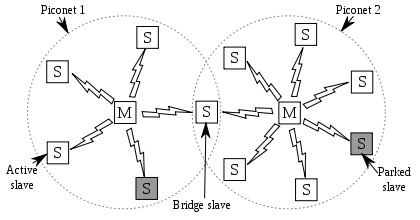
\includegraphics[width=\linewidth]{Kapitel/Bluetooth_4/Grafiken/piconetz.png}
\captionof{figure}{zwei Piconetze durch einen Bridge-Knoten zu einem Scatternetz verbunden \cite{Bluetooth_4.3} }
\label{fig:bt4.scatternetz}
\end{Figure}

\subsubsection*{Übertragungsverfahren}
Die Übertragung von Daten erfolgt über die Funkschicht. Bluetooth benutzt dafür das \textbf{ISM}-Band (\textbf{I}ndustrial, \textbf{S}cientific, \textbf{M}edical) im 2,4~GHz-Bereich. Daraus ergeben sich 79 Kanäle mit je 1~MHz Bandbreite. Da jedoch das ISM-Band auch von anderen Netzen verwendet wird, kann es zu Störungen kommen. Um dies zu verhindern, wird bei Bluetooth eine Frequenzsprungtechnik mit Spektrumsspreizung verwendet. Es können bis zu 1600 Sprünge in der Sekunde über Zeitscheiben mit einer Dauer von 625 Mikrosekunden geschehen. In einem Piconetz springen alle Knoten zur gleichen Zeit und richten sich nach der Zeitscheibenvorgabe und Sprungfolge des Masters. Da sich Übertragungen früherer Versionen von Bluetooth und IEEE 802.11-Übertagungen gegenseitig zerstören (Abb. \ref{fig:bt4.ueberlagerung}), wurde die Frequenzsprungfolge so verändert, dass sie Kanäle auslassen, auf denen andere Radiofrequenz-Signale existieren, um die schädlichen Interferenzen zu verkleinern. Diese Methode wird als adaptives Frequenzsprungverfahren (Abb.~\ref{fig:bt4.verfahren}) bezeichnet. \cite{Bluetooth_4.2}

\begin{Figure}
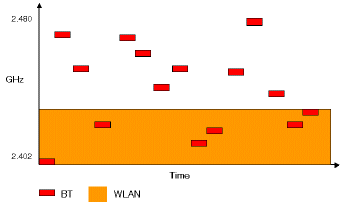
\includegraphics[width=\linewidth]{Kapitel/Bluetooth_4/Grafiken/kollisionen.png}
\captionof{figure}{Überlagerungen zwischen Bluetooth und IEEE 802.11 \cite{Bluetooth_4.5} }
\label{fig:bt4.ueberlagerung}
\end{Figure}

\begin{Figure}
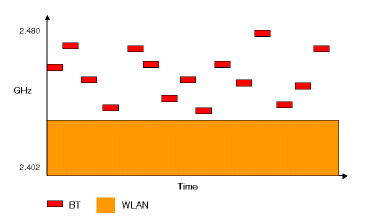
\includegraphics[width=\linewidth]{Kapitel/Bluetooth_4/Grafiken/frequenzsprung.png}
\captionof{figure}{Lösung durch das adaptive Frequenzsprungverfahren \cite{Bluetooth_4.5} }
\label{fig:bt4.verfahren}
\end{Figure}

\subsubsection*{Rahmenstruktur}
Unter "Rahmen" versteht man in diesem Umfeld den Protokollrahmen, d.h. den Aufbau der Pakete, die zwischen Bluetooth-Geräten ausgetauscht werden. Zwei wichtige Rahmenformate von Bluetooth sind in Abb. \ref{fig:bt4.rahmenstruktur} dargestellt. Den Anfang eines jeden Rahmens bildet ein Zugriffscode, der den Master bestimmt. Dadurch können Slaves in der Reichweite von zwei Master-Knoten ermitteln, welche Daten für sie bestimmt sind. Es folgt ein 54-Bit-Header mit den gleichen Feldern, die auch für die MAC-Teilschicht im OSI-Modell typisch sind. 

Widmen wir uns kurz dem Header. Das Adress-Feld gibt an, für welches Gerät im Piconetz der Rahmen bestimmt ist. Das Feld Type spezifiziert den Rahmentyp (z.B. Polling), die Anzahl der Zeitscheiben, die der Rahmen umfasst, und die Art der Fehlerkorrektur, die im Datenfeld angewendet wird. Darauf folgen drei Flags. Das Flow-Bit kann von einem Slave-Knoten gesetzt werden, um anzuzeigen, dass sein Speicher voll ist und er keine Daten mehr empfangen kann. Das Acknowledgement-Bit dient der Mitsendung einer Bestätigung in einem Rahmen. Das Sequence-Bit wird zur Nummerierung von Rahmen verwendet, um redundante Übertragungen zu erkennen. Schließlich folgt eine Prüfsumme von 8~Bit.

Wenn der Rahmen mit der Basisdatenrate gesendet wird, folgen auf den Header die Daten. Das Datenfeld kann abhängig davon, über wie viele Zeitscheiben die Übertragung stattfindet, 0-2744~Bit lang sein. Falls der Rahmen mit erweiterter Datenrate gesendet wird, kann das Datenfeld bis zu zwei- oder dreimal so viele Bits besitzen. Den Daten ist dann ein Sicherheitsfeld und ein Synchronisationsmuster vorangestellt. Die Aufgabe des Synchronisationsmusters ist es, auf die schnellere Datenrate umzuschalten, da bei erweiterter Datenrate der Adresscode und der Header dennoch mit Basisrate und nur die Daten mit erweiterter Datenrate gesendet werden. Üblicherweise werden Rahmen mit erweiterter Datenrate mit einem Trailer abgeschlossen. \cite{Bluetooth_4.2}

\begin{Figure}
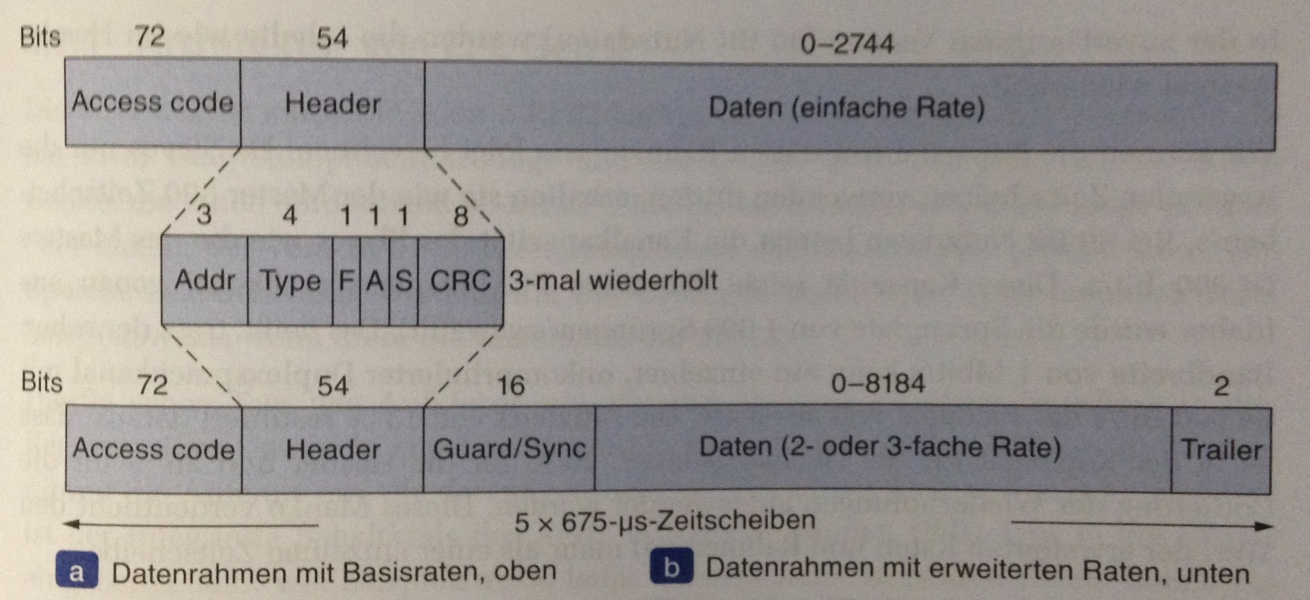
\includegraphics[width=\linewidth]{Kapitel/Bluetooth_4/Grafiken/rahmenstruktur.jpg}
\captionof{figure}{Überblick über die Rahmenstruktur in Bluetooth \cite{Bluetooth_4.2}
}
\label{fig:bt4.rahmenstruktur}
\end{Figure}

\end{multicols}
\newpage
\section*{Historische Entwicklung}
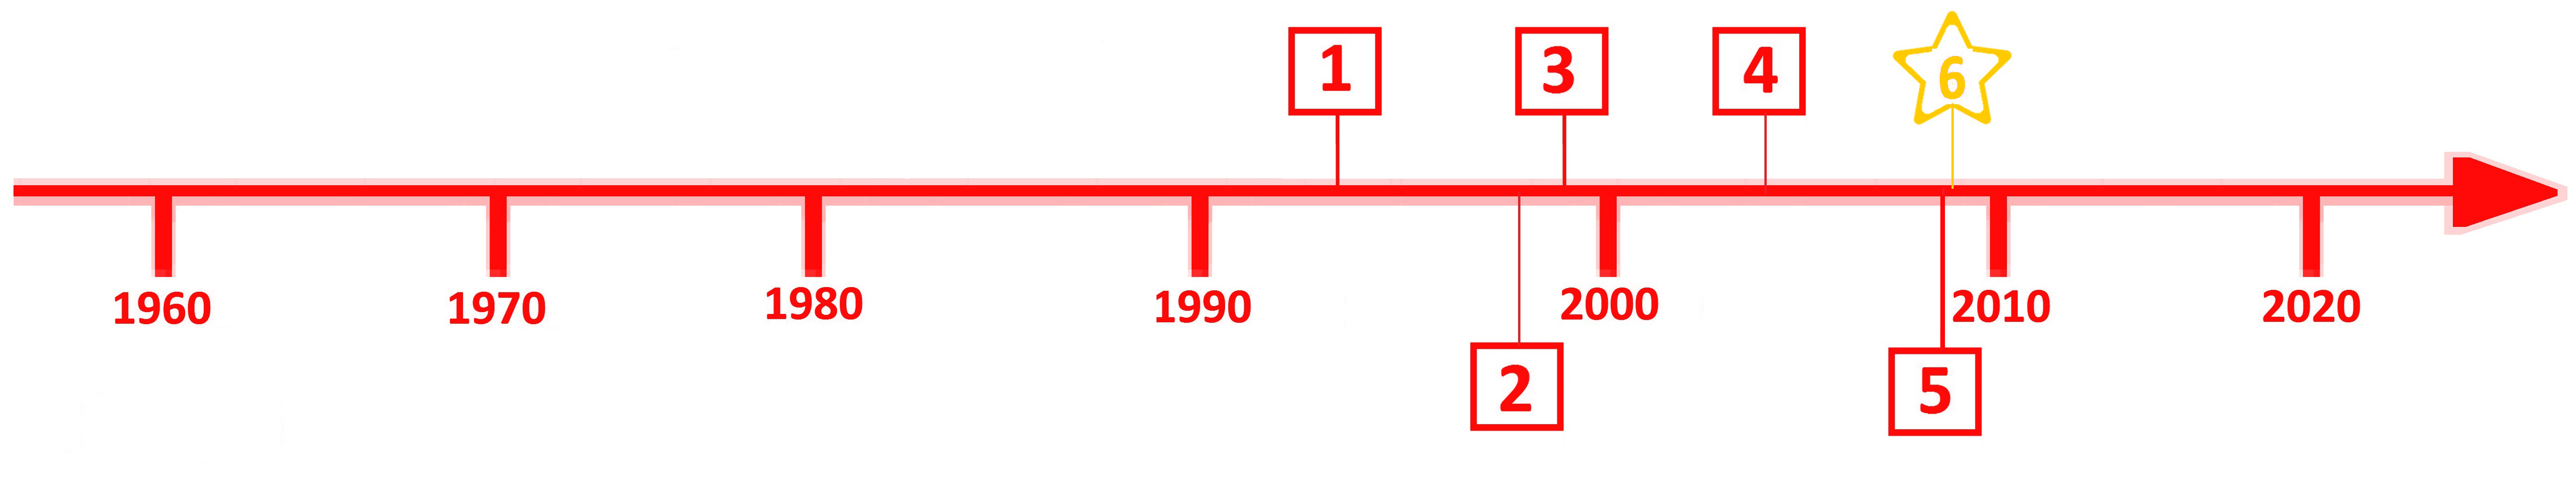
\includegraphics[width=\textwidth]{Kapitel/Bluetooth_4/Grafiken/Zeitstrahl.jpg}
\par
\noindent
\rowcolors{2}{}{\topicolor!20}
\begin{tabular}{p{0.5 cm}p{1.5 cm}p{15.55 cm}}
	Nr. & Datum & Entwicklungsschritte~\cite{Bluetooth_4.2}\\
	1 & 1994 & Das Unternehmen L.M.Ericsson beginnt mit der Entwicklung einer Technologie für kabellose Verbindungen zwischen Mobiltelefonen und anderen Geräten.\\
	2 & 1998 & Bildung der Bluetooth \textbf{SIG} (\textit{\textbf{B}luetooth \textbf{S}pecial \textbf{I}nterest \textbf{G}roup}) mit vier anderen Unternehmen, um einen drahtlosen Standard zur Verbindung von Rechnern und Kommunikationsgeräten zu spezifizieren.\\
	3 & Juli 1999 & Veröffentlichung von Bluetooth 1.0\\
	4 & 2004 & Nachdem die Protokolle aus Version 1.0 stabil laufen werden diese mit höheren Datenraten zu Bluetooth 2.0 ergänzt.\\
	5 & 2009 & Mit der dritten Version von Bluetooth werden in Kombination mit IEEE 802.11 Datenübertragungen mit höherem Durchsatz möglich.\\
	6 & Dezember 2009 & Veröffentlichung der Spezifikation für Bluetooth 4.0, die Niedrigenergie-Betrieb inkludiert\\
\end{tabular}
\par
\begin{multicols}{3}

\subsubsection*{Neuerungen von Bluetooth 4.0}
Man spricht bei Bluetooth in der Version 4.0 auch von Bluetooth \textbf{L}ow \textbf{E}nergie (\textbf{LE}). Der Name leitet sich davon ab, dass es sich um eine, im Gegensatz zu seinen Vorgängern, sehr stromsparende Version handelt. Dadurch ergeben sich nun Anwendungsmöglichkeiten auf Geräten, bei denen bisher die Batterie für den Betrieb von Bluetooth nicht ausgereicht hätte. Low-Energy-Geräte ab Bluetooth 4.0 sind speziell für Anwendungen ausgelegt, die in größeren Intervallen kleine Datenmengen übertragen. Reine Low-Energy-Geräte sind beispielsweise Smartwatches, Sportsensoren oder Aktivitätstracker, die mit einem Smartphone gekoppelt sind. Bluetooth 4.0 ist allerdings nur bedingt zu früheren Versionen kompatibel. Ein Gerät, dass nur Bluetooth 4.x kennt, setzt bei seiner Gegenstelle ebenfalls Bluetooth 4.x voraus. \cite{Bluetooth_4.6}

\subsection*{Einsatz}
Die Bluetooth SIG spezifiziert Anwendungen, die unterstützt werden sollen und stellt für jede Anwendung eine Reihe von Protokollen bereit. Es existieren eine ganze Reihe von Anwendungen bzw. sogenannten „Profilen“. Im Folgenden werden zunächst ausgewählte Profile und ihre Anwendungen vorgestellt, die nicht mit Bluetooth 4.0 spezifiziert wurden, sondern mit älteren Versionen. Diese wurden jedoch in der 4.0-Spezifikation übernommen und mit neuen Profilen ergänzt. Einige Profile sind für die Übertragung von Audio und Video vorgesehen. Ein Beispiel ist das \textbf{I}nter\textbf{c}ommunication\textbf{p}rofile (\textbf{ICP}), welches es ermöglicht, zwei Telefone als Walkie-Talkies zu verbinden. Dazu kommen Headset- und Freisprechprofile, um Peripheriegeräte wie Headsets mit einer Basisstation zu verbinden. Andere Profile regeln das Streamen von Audio- und Videodaten in Stereoqualität, beispielsweise von einem Handy auf einen tragbaren Lautsprecher oder von einer Kamera auf einen Fernseher.

Außerdem existieren Profile zum Verbinden von Tastaturen und Mäusen an einen PC (HID), um ein Handy als Fernbedienung für einen Bluetooth-fähigen Fernseher zu verwenden oder Profile, die Netzbetrieb ermöglichen. Zu letzteren gehört zum Beispiel das PAN-Profil, mit dem Bluetooth-Geräte ein Ad-hoc-Netz bilden können oder das \textbf{DUN}-Profil (\textbf{D}ial-\textbf{U}p \textbf{N}etworking), durch das sich ein Notebook kabellos mit einem Handy verbinden kann, das ein Modem enthält. Erwähnenswert ist das \textbf{G}eneric-\textbf{Att}ribute-Profil (\textbf{GATT}), das für die neue Version Bluetooth 4.0 spezifiziert wurde. Es wird als Master-Profil für andere Profile verwendet, um kleine Datenmengen energieeffizient zu übertragen. \cite{Bluetooth_4.2}

\subsection*{Anbieter und Gremien}
Für die Bluetooth-Technologie, einschließlich der Version 4.0, ist die Bluetooth SIG zuständig. Diese wurde 1998 von 5 Unternehmen gegründet und war im März 2015 bereits eine Interessengemeinschaft von mehr als 8000 Unternehmen, die bei der Entwicklung und Verbreitung der Technologie zusammenwirken. Die Bluetooth SIG ist darüber hinaus auch der Eigentümer des Bluetooth-Zeichens und Herausgeber der Bluetooth-Spezifikation. \cite{Bluetooth_4.4}

\subsection*{Ausblick}
Die Bluetooth-Technologie ist heute für das kabellose 
Verbinden von verschiedenen Geräten unerlässlich geworden. 
Das gilt sowohl für die älteren Spezifikationen als auch für 
Bluetooth 4.0, durch das völlig neue Einsatzgebiete möglich werden. 
Dies betrifft vor allem den Betrieb auf kleinen Geräten, für die 
Bluetooth-Anwendungen bisher, aufgrund des hohen Energieverbrauchs,
nur bedingt nützlich waren. Meiner Meinung nach ist die Technologie
von Bluetooth sehr interessant und es ist lohnenswert sich damit einmal
genauer zu befassen, zumal fast jeder von uns Bluetooth schon einmal benutzt hat. 
Darüber hinaus bleibt es spannend zu verfolgen, inwiefern sich Bluetooth 4.0 
und seine Einsatzgebiete in den nächsten Jahren entwickeln werden.
\printbibliography[segment=3,heading=subbibliography]
\end{multicols}

\newpage
